%\section{Graphical Query Composition}
%\label{sec:gui}

\begin{figure*}[th!]
\centering
\begin{minipage}{3.2in}
  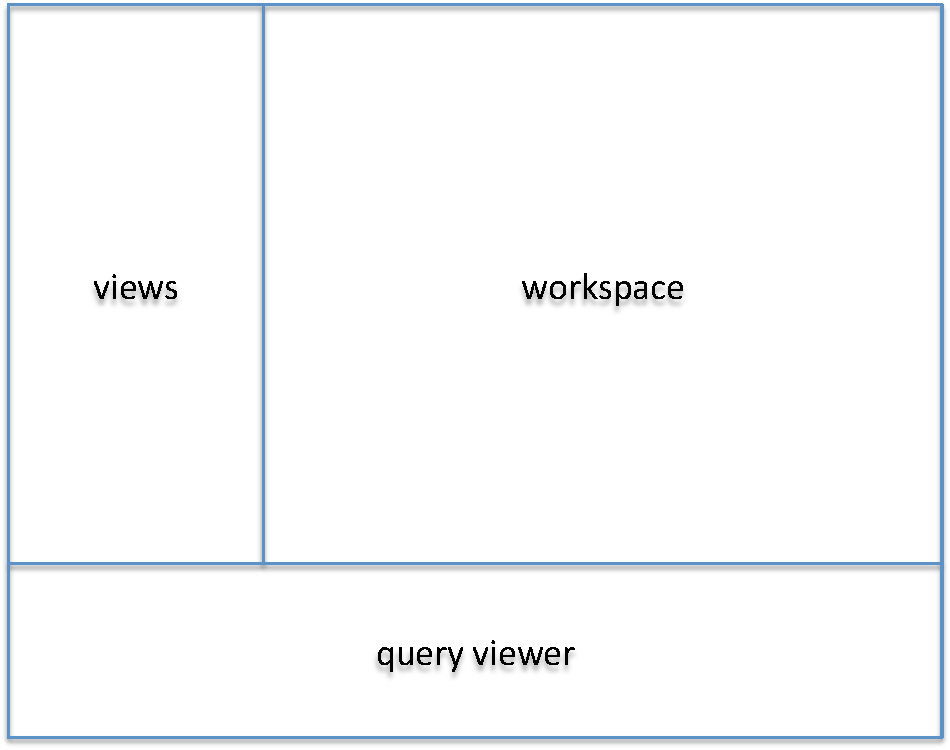
\includegraphics[width=2.9in]{figs/ui.pdf}
  \caption{Graphical query composition. PLACEHOLDER}
  \label{fig:ui}
\end{minipage}
\begin{minipage}{3.2in}
  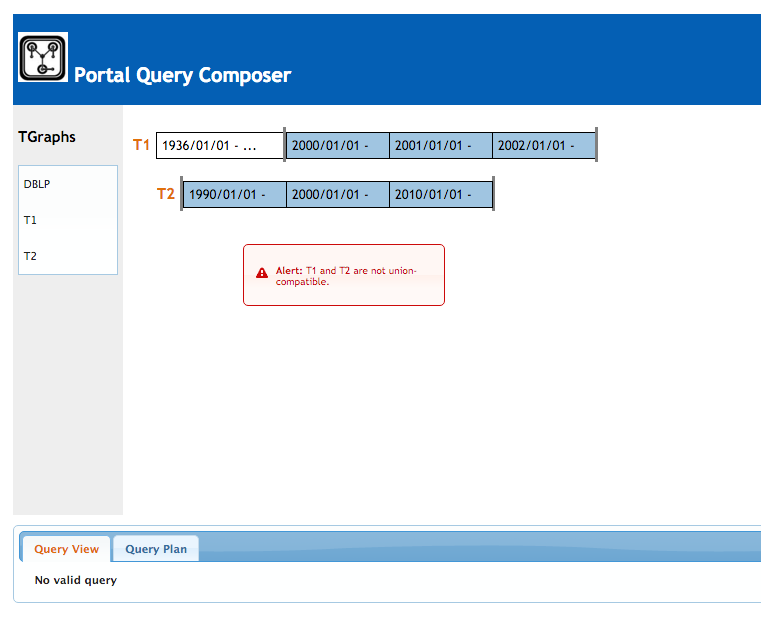
\includegraphics[width=2.9in]{figs/uierror.png}
  \caption{Union compatibility assistance. PLACEHOLDER}
  \label{fig:uierror}
\end{minipage}
\end{figure*}

{\bf Graphical query composer.} Evolving graph analysis is of interest
to researchers in many domains.  While \ql is declarative and, thus,
does not require computer science expertise to use, we want to reach a
wide audience.  For this reason, we are developing a web-based
graphical query composition tool \qlui (Figure~\ref{fig:ui}).

\qlui users can compose queries by adding to and manipulating \tg{}s
in the workspace, where they are represented by their timelines.  To
select a temporal subset of a \tg, the user can move the outside
border of the timeline.  To aggregate a \tg, the user can move the
border of any of the timeline periods and then specify the aggregation
functions through a drop-down menu.

As the query is composed graphically, its \ql representation is
updated in the Query view.  The user can also view the optimized plan
for the query in the Plan view and execute it in the integrated Shell.

To temporally join two \tgs, the user can drag them to the workspace
and place them close together.  Two \tgs can only be joined if they
are {\em union-compatible}, that is, if their temporal sequences have
the same resolution and can be aligned.  If the two graphs are not
union-compatible, they will not snap together and an error message is
displayed to the user explaning the problem, as can be seen in
Figure~\ref{fig:uierror}.  Union-compatibility is one of the more
complex aspects of the language, and it is our hope that a graphical
representation of the \tg temporal schema will reduce confusion.


